\documentclass[conference]{IEEEtran}

\usepackage{epsfig}
\usepackage{fancyvrb}

\DefineVerbatimEnvironment%
  {code}{Verbatim}{numbers=left,numbersep=3pt,frame=lines,%
                   xleftmargin=7pt,fontsize=\footnotesize}




\begin{document}


\title{An OSGi-based Sensor Network for \\ Environmental Monitoring}

\author{\authorblockN{A. Puder, T. Johnson, K. Sales, M. Sales}
\authorblockA{San Francisco State University \\
Computer Science Department \\
1600 Holloway Avenue \\
San Francisco, CA 94132 \\
EMail: \{arno$\mid$tlj$\mid$klebers$\mid$msales\}@sfsu.edu}
\and
\authorblockN{D. Robinson}
\authorblockA{San Francisco State University \\
Romberg Tiburon Center \\
3150 Paradise Drive \\
Tiburon, CA 94920 \\
EMail: dhr@sfsu.edu}}


\maketitle
\begin{abstract}
  Abstract.
\end{abstract}


\section{Introduction}

\cite{roemer:2004}

Environmental monitoring depends on the reliable collection of
measurements from remotely deployed sensors and the rapid transfer of
those measurements to data centers where processing and analysis may
take place. Typically, sensors are deployed in out-of-the-way
locations where physical access is limited and connections for
telemetry are poor or nonexistent.   Maintaining the data stream from
these sensors places demands on human resources, requiring site visits
to service the sensors and to download data stored on internal memory.
Consequently, there is a lag of days to months between the time the
sensors perform the measurements and the time the measurements becomes
available.   Advances in battery life and anti-fouling technology have
extended service cycles for field sensors, with the unwanted result of
further delaying access to monitoring data.  In addition, the
dependence on field site visits to alter of sensor characteristics,
such as sampling rate, prevents adjustment in monitoring strategy in
response to rapidly developing events (e.g. oil spills, harmful algal
blooms).

To address these problems of data collection from remote
sensors, we propose to develop an automated end-to-end system based on
proven technology that provides a means to program and interrogate
sensors at the remote field locations and to transmit collected
measurements over long distances to data collections centers where the
data is rapidly processed, archived, and made available to potential
users in near real-time.


\section{Background}

Researchers in the geosciences rely on sensor data collected by highly
specialized sensors such as the Seabird or YSI. These sensors are
usually deployed in remote locations that not only make their
maintenance difficult, but also access to their measurements.
Typically the sensors are autonomous in the sense that they can run
for a certain time on battery power and store the measurement data in
internal memory. Only when the sensors are serviced, the measurement
data they have collected since the last servicing are uploaded to a
portable storage device. From there the data can be uploaded to
server. This manual procedure to retrieve sensor data is not only
error prone, but also results in a serious time lag between the time
the sensor performs the measurement and when it becomes available for
further processing. For many applications it would be beneficial to
have near-realtime access to the sensor measurement. Being able to
access data when they become available on the sensor device also
reduces the maintenance overhead.

---

The YSI 6600EDS V2 Sonde is a water quality monitoring device that
gathers water quality data, and operates in fresh, sea, or
polluted water. It is under 22 inches (under 55 cm) in length, 3.5
inches (8.9 cm) in diameter, and weighs approximately 7 pounds (3.18
kg). It operates at temperatures between -5 to +50 deg C and at depths
up to 656 feet (200 meters).  It uses 8 C-size Alkaline Batteries or
External 12 VDC. Battery life can last up to 75 days depending on
sensor configuration. The Sonde's bulkhead contains multiple pin
connectors to support sensor probes for measuring the following:

\begin{table}[h]
\caption{\label{TAB_SONDE_MEASUREMENTS} YSI Sonde measurements.}
\centering
\begin{tabular}{|l||l|}
\hline
\multicolumn{1}{|c||}{\textbf{Name}} &
\multicolumn{1}{c|}{\textbf{Description}} \\ \hline \hline
\texttt{Date}    & Year/Month/Day. \\ \hline
\texttt{Time}    & Hour:Minute:Second. \\ \hline
\texttt{Temp}    & Temperature in degrees Celcius. \\ \hline
\texttt{SpCond}  & Specific Description in microSiemens
                   per centimeter. \\ \hline
\texttt{Cond}    & Conductivity in microSiemens per centimeter. \\ \hline
\texttt{Resist}  & Resistivity in Ohms $*$ centimeter. \\ \hline
\texttt{Sal}     & Salinity in parts per thousand. \\ \hline
\texttt{Press}   & Pressure in pounds per square inch relative. \\ \hline
\texttt{Depth}   & Water column in meters. \\ \hline
\texttt{pH}      & pH in standard units. \\ \hline
\texttt{phmV}    & millivolts associated with the pH reading. \\ \hline
\texttt{ODOSat}  & Dissolved oxygen in \% air saturation. \\ \hline
\texttt{ODOConc} & Dissolved oxygen in mg/L. \\ \hline
\texttt{Turbid}  & Turbidity in nephelometric turbidity units. \\ \hline
\texttt{Battery} & Total Volts remaining in batteries.  \\ \hline
\end{tabular}
\end{table}

Dissolved oxygen
Conductivity/Temperature
Fouling Resistant pH/ORP
Chloride
Ammonium
Nitrate
Turbidity
Chlorophyll
Rhodamine
PC-Blue-green Algae
PE-Blue-gren Algae

Each probe may have multiple sensors.  A computer can interface with
the Sonde via RS-232C or SDI-12. The Sonde can be configured to
collect data samples in discrete or unnattended mode.  Discrete mode
is normally performed while a technician manages the Sonde during the
sampling process. In this mode the Sonde is usually connected via 650
MDS Display/Logger or a serial cable connected to a PC.  The sampling
frequency is usually set to a high frequency in this mode.  Unattended
mode is performed usually when the Sonde is deployed offshore or in a
remote body of water.  The sampling frequency is usually set for a
longer period of time (i.e. 5 - 15 min). The Sonde is configured via a
set of menus that can be accessed through a terminal session over
RS232. Through these menus, the Sonde can be configured to start
logging data to an internal file.  To view the data as it's being
captured, the option to show live data is chosen and the data can then
seen via a serial terminal session at each interval.

---

Start with some related work. Who else has done an OSGi-based
infrastructure for sensor networks? Kleber: I believe you have a few
references. This section should be a combination of a use case (using
the RTC and their YSI sonde as an example) and a requirements
analysis: requirements such as remote management and monitoring
capabilities, time-delayed communication, etc. In this section should
be no mentioned of DSP or OSGi. Length: 1 page.

\section{Data Sensor Platform}

Should describe the OSGi-based NetBEAMS architecture. Total length of
this section: 2 pages.

Micro-kernel architecture.

\subsection{Architecture}

Our architecture is based on a micro-kernel approach. The core
functionality is limited to a minimum and all extra services are built
as plug-and-play modules on top of the micro-kernel. With the help of
this approach we can keep the basic infrastructure compact while
allowing customization via special-purpose modules. In our terminology
we call the basic foundation the \emph{Data Sensor Platform}
(DSP). The scope of the DSP is one address space of an execution
platform. A sensor network is built from several DSPs that are linked
with each other.

Figure \ref{FIG_DSP} depicts the basic architecture of the
DSP. We refer to the plug-and-play modules as DSP Components. DSP
Components are self-contained modules that can be added and removed to
a DSP installation at runtime. The basic communication paradigm within
a DSP is a message. DSP Components can exchange messages of different
types. We distinguish between Data Producers (DP) and Data Consumers
(DP) within the scope of a DSP. DP and DC can be seen as roles that a
DSP Component may have. It is possible for a DSP Component to act in
the role of DC and DP at the same time.


\begin{figure}
\centering
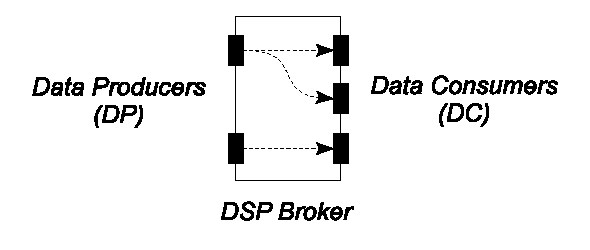
\epsfig{file=dsp, width=7cm}
\caption{\label{FIG_DSP} Data Sensor Platform (DSP).}
\end{figure}

The DSP is responsible for routing messages between DPs and DCs. It is
important to note that this routing only happens withing a
DSP. Following the paradigm of a micro-kernel approach, the DSP has no
notion of remote communication or sensor-specific details. All this
knowledge is embodied in DSP Components.

\subsection{Components}

Should give some API sniplets for DP and DC.

\begin{code}
interface DSPComponent
{
   public String getComponentType();
   public void initComponent(...);
   public void startComponent();
   public void stopComponent();
   public void deliver(DSPMessage msg);
   public Message deliverWithReply(DSPMessage msg);
   // ...
}
\end{code}


\subsection{Message}

\begin{code}
<xs:schema ...>
  <xs:complexType name="DSPMessage">
    <xs:element name="Header" type="Header"/>
  </xs:complexType>

  <xs:complexType name="Header">
    <xs:sequence>
      <xs:attribute name="messageID"/>
      <xs:attribute name="originatingDP"/>
      <!-- ... -->
    </xs:sequence>
  </xs:complexType>
</xs:schema>
\end{code}

Should explain the way DSP Messages are defined: XML Schema and JAXB.

\subsection{Matcher}


\section{NetBEAMS}

In the following we present a practical application the the DSP
presented in the previous section. We describe a deployment of the DSP
using sensor owned and operated by the RTC. Our environmental sensor
network is dubbed NetBEAMS (Networked Bay Environmental Assessment
Monitoring System) and allows access to sensor equipment deployed
throughout the San Francisco Bay Area. Figure \ref{FIG_NETBEAMS}
provides an end-to-end overview of the NetBEAMS architecture. NetBEAMS
is built using multiple installtion of the DSP. One DSP installation
is collocated with each sensor and an additional DSP is running on the
backend server.

\begin{figure*}
\centering
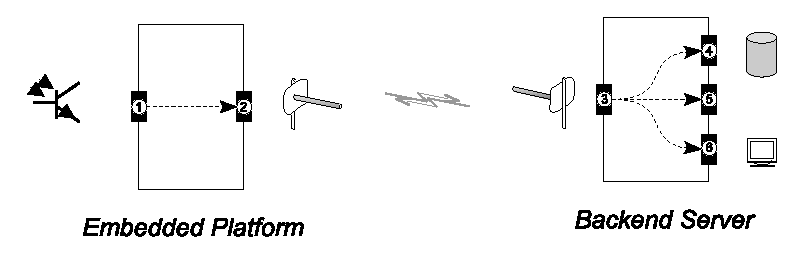
\epsfig{file=netbeams, width=14cm}
\caption{\label{FIG_NETBEAMS} NetBEAMS architecture.}
\end{figure*}

To describe NetBEAMS is to describe the specific DC and DP we have
implemented. On the far left of Figure \ref{FIG_NETBEAMS} is the
actual sensor; in our case the aforementioned Seabird sensor.
Collocated with the Seabird is an embedded system. Here we make use of
a platform called Gumstix. 

The Gumstix is a single-board computers with 256 Mb of flash and 256
Mb of SDRAM, and running a 600 MHz TI OMAP 3503 processor. Additional
features can be added to the motherboard with expansion cards
connected via on-board buses. The motherboards draw less than 250 mA
@4V at 400 MHz and less than 50 mA while idling, waiting for input.
Gumstix run Linux 2.6 with the BusyBox utilities, and use the
OpenEmbedded build environment to provide a complete Linux
environment and a large range of Linux applications. We use the JamVM
implementation of Sun Microsystem's virtual machine to execute Java
programs. 

The Huawei E220 is a USB modem that supports HSDPA, UMTS, EDGE packet
data services at maximum transmission rates of 3.6Mbps, 384kbps, and
236.8kbps respectively. HSDPA and UMTS operate at 2100MHz while GSM,
GPRS, and EDGE operate at 900, 1800, and 1900MHz. The modem connects
to the Verdex Pro XM4 motherboard via a mini USB interface (supporting
USB 2.0). Linux kernels since 2.6.20 include support for E220 drivers.
This includes the linux kernel on the gumstix which runs 2.6.21.  The
gumstix communicates with the modem using the PPP protocol and
accesses the cellular network using a data plan from AT\&T.



\subsection{YSI Sonde DP}

\begin{code}
<xs:schema ...>
<xs:import schemaLocation="dsp-message.xsd"/>

<xs:element name="SondeDataMessage">
  <xs:complexType>
    <xs:complexContent>
      <xs:extension base="DSPMessage">
        <xs:sequence maxOccurs="unbounded"
                     minOccurs="1">
          <xs:element name="sondeData"
                      type="sondeDataType"/>
        </xs:sequence>
      </xs:extension>
    </xs:complexContent>
  </xs:complexType>
</xs:element>

<xs:complexType name="sondeDataType">
  <xs:sequence>
    <xs:element name="Date" type="xs:date"/>
    <xs:element name="Time" type="xs:time"/>
    <xs:element name="Temp" type="xs:float"/>
    <xs:element name="SpCond" type="xs:float"/>
    <!-- ... -->
  </xs:sequence>
</xs:complexType>
</xs:schema>
\end{code}

\subsection{Wire transport DC/DP}

\subsection{Web Managements}


\section{Conclusions and Outlook}

Length (including bibliography): 0.5 pages.

The California coastal region is populated by a vast number of
remotely deployed sensors that monitor environmental conditions
ranging from weather to water quality to ocean surface currents.
These sensors are operated by data providers, including resource
management groups, research scientists, municipalities, and state and
federal agencies, who could use near real-time data streams to inform
decision that impact public health, public safety, and the protection
of resources.  In addition, there are efforts underway at the state
and federal level to collate the data collected by the individual data
providers into integrated monitoring networks that will enhance the
distribution of monitoring data to public, private, and federal users
groups.  Success of these efforts, whether small scale or a large
integrated network, depends on the first step in the data management
process: reliably obtaining data in near real-time from remotely
located sensors.  This step can be the weak link in the data
management pathway when telemetry options are unreliable.  The
availability of a plug-and-play computing platform designed to
communicate with a variety of sensor types and to provide data
telemetry to distant brick and mortar data centers would stabilize
data streams with poor telemetry and allowing expansion of sensor
coverage into regions not presently served.  The low power consumption
and low cost of these units would be particularly beneficial for
applications with long service cycles and for data providers trying to
maintain data streams on a limited budget.

\bibliography{lit}
\bibliographystyle{plain}


\end{document}
